\documentclass[a4paper]{article}
\usepackage[utf8]{inputenc}
\usepackage[english]{babel}
\usepackage{amsmath,amsthm,amssymb}
\usepackage{geometry}
\usepackage{braket}
\usepackage{tikz}
\usepackage{placeins}

\newcommand{\HH}{\mathcal{H}}

\title{Mangled Children \\ \large Quantum exploration of a classical epistemic
 puzzle}
\author{Krasimir Georgiev}

\begin{document}
\maketitle
\section*{Introduction} The muddy children puzzle is a well-known epistemic
puzzle that illustrates some features of the dynamics of knowledge. 
Quantum physics is normally perceived as a notoriously unintuitive
discipline. It lacks connections with real world intuitions and has bizzarre
predictions. In this report we construct quantum analogues of the muddy
children puzzle. We explore these variants using a blend of quantum and
epistemic logic.

\section*{Muddy children} The  muddy children puzzle goes as follows:
several clever (logically omniscient) children are playing with mud; their
father comes and publicly announces that some of the children have mud on
their face. Then he asks the same question over and over again: Do you know if
you are muddy? Each child publicly announces the answer truthfully at the same
time. Of course, each child sees everyone else's faces except for its own. What
happens is the following: during first several rounds, each child answers
negatively. But at some specific round, exactly the muddy children answer
positively. At first sight this is paradoxical: by listening to the same answers
of the same question over and over again, the children come to learn new
information.

For $n$ children, we may model the puzzle by an epistemic model where the worlds
are all the strings over $\{0, 1\}$ of length $n$, where $1$ at position $i$
denotes that the $i$-th child has mud on its face.
The indistinguishability relation $R_i$ for the $i$-th child contains all the
pairs of strings that possibly differ only at the $i$-th position.
Suppose that $u \geq 1$ of the children are actually muddy. The public
announcement of the father effectively deletes the world $0^n$. At round $r = 1,
2, \dots, u-1$, the public announcements of the children delete all the worlds
having $r$ ones.  At round $r = u$, since all worlds with a lower number of ones
are deleted, all the muddy children can distinguish the real world, so they give
a positive answer.

\section*{Quantum world}

The postulates of quantum physics tell us that the possible states of a quantum
system correspond to the one-dimensional (closed) subspaces of a Hilbert space
$\HH$. Equivalently (up to a complex multiple), the states may be represented by
nonzero vectors. Quantum evolution of the system is captured by an unitary
operation on $\HH$. Only the properties corresponding to the closed subspaces $S
\subseteq \HH$ are physically observable and a quantum test has a probabilistic
ontic effect on the system. Suppose we test the property $S$ at a state
represented by the unit vector $s \in \HH$. We have $s = s^{\perp} +
s^{\parallel}$ for some $s^{\perp} \perp S$ and $s^{\parallel} \in S$ (we will
always assume this when $S$ is clear from the context). There are
two possible outcomes. With probability $|s^{\parallel}|^2$ the test would have
a positive outcome and the system will collapse to the state $s^{\parallel}$.
Similarly, with probability $|s^{\perp}|^2 = 1 - |s^{\parallel}|^2$ the test
would have a negative outcome and the system will collapse to the state
$s^{\perp}$. In a sense, the observations act like public announcements that
collapse the quantum system to a state that is consistent with the outcome of
the answers. There is the property of repeatability, which says that quantum
observations are idempotent, but in general we lack monotonicity, because a
sequence of observations typically changes the real world quantum state.

We have to reconsider parts of the muddy children puzzle in this quantum
setting. We start by thinking of the mud on the faces of the children as some
kind of a quantum system. Then the act of determining if a child has muddy face
amounts to performing a quantum observation. Thus, in the general quantum case, 
it no longer makes much sense to consider absolute, classical propositions like:
``you are muddy''. Instead, it is more natural to consider dynamic
versions of this statement. 
Suppose the real world quantum state corresponds to the unit vector $s \in \HH$,
and suppose that the observation corresponds to the closed subspace $S \subseteq
\HH$. The following are versions of the statement:
\begin{itemize}
\item \emph{After observation, you will possibly be (become) muddy}. This
    corresponds to $s \not\perp S$.
\item \emph{After observation, you will surely be (become) muddy}. This
    corresponds to $s \parallel S$.
\item \emph{After observation, you will be muddy with probability $P \in [0,
    1]$}. This corresponds to $|s^{\parallel}|^2 = P$ and is a generalization of
    the previous two versions.
\end{itemize}

Note that these statements are impractical for direct verification. In
principle, one needs an infinite amount of identical quantum system copies of
$s$ to estimate the probability of the outcomes of the observation, since each
state collapses after being observed.

We will assume further that the father is a quantum omniscient entity, having
access to the full information about the quantum system \emph{without disturbing
it}. Their father plays a god role in the quantum versions of the puzzle.

The next issue is the issue of quantum disjunction. Namely, we are concerned in
interpreting the initial announcement of the father: someone is muddy. Since the
union of closed subspaces is not necessarily a closed subspace, in general the
classical version of that statement does not correspond to an observable
property of the system. In the next section, we will analyze a version of the
puzzle in which the property \emph{after observation, it is impossible that
everyone is clean} happens to be a testable property. There is a weaker form of
quantum disjunction that is interpreted by the span of the interpretation of the
classical disjunction. We see a setting in which this quantum disjunction is too
weak to give the children any new information whatsoever. Note that there is no
such issue occurring with (quantum) conjunction, since the intersection of
closed subspaces is itself a closed subspace.

Another issue that pops up is the simultaneous observations. Since an
observation has an ontic effect, it is in general impossible for all observers
to observe the system at the same time. Only in specific cases (as in the next
section) simultaneous observations will make sense. When this might lead to
problems, we will number the children by $1, 2, \dots, n$ and assume (that it is
public knowledge) that they make their quantum observations in that order. Note
that this does not necessarily imply a restriction to their simultaneous
classical answer to the question of the father.

Finally, the question of the father needs to be adapted so that it blends the
quantum and epistemic features of the situation. We will consider variants of 
the following plausible adaptation:
\emph{After you did the quantum observation (that you were supposed to do,
    typically observing the others), do you know that if your face is observed,
it will (possibly/surely) be dirty?}


\section*{Composite qubit system}
For our first concrete version of the puzzle, let us consider a situation in
which there are just $n = 2$ children: Alice and Bob. There is a qubit
representing the cleanliness of each one's face. Alice's face has two possible
observable states: $\ket{a}$, in which case she is clean, and $\ket{A}$, in
which case she is dirty. Similarly for Bob the states are $\ket{b}$ and
$\ket{B}$. A general state of this quantum system corresponds to a unit vector
$s$ in the four-dimensional Hilbert space $\HH$ with orthonormal basis $\{\ket{ab},
\ket{aB}, \ket{Ab}, \ket{AB}\}$ and we may write it as $s = \alpha \ket{ab} +
\beta \ket{aB} + \gamma \ket{Ab} + \delta \ket{AB}$, $\alpha, \beta, \gamma,
\delta \in \mathbb{C}, |\alpha|^2 + |\beta|^2 + |\gamma|^2 + |\delta|^2 = 1$.
Assume that this is common knowledge, so our initial epistemic model contains
all of these $s$ and the indistinguishability relations $R_i$ are the full
relations over the state space.
Now the father tells them: \emph{it is impossible that after an observation of
both of you, both of you are clean}. Note that this is a yet another variant of
the initial announcement that can be formulated in this particular setting. It
is true iff $\alpha = 0$. The public announcement of this statement effectively
deletes the states having $\alpha \neq 0$ from the epistemic model, leaving us
with a general state of the epistemic model as $s = \beta\ket{aB} +
\gamma\ket{Ab} + \delta\ket{AB}$.

Now the father asks the children if they know that they are dirty, or more
precisely, if after having observed the other child, they came to know that if
their face is observed, it will surely be dirty. First Alice observes Bob's
face and by doing so, she collapses the system to a state that is consistent
with her observation. In detail:
\begin{enumerate}
    \item She might observe that Bob is muddy (which happens with probability
        $|\beta|^2 + |\delta|^2$). In that case the system collapses to the state
        $s' = \frac{\beta\ket{aB} + \delta\ket{AB}}{\sqrt{|\beta|^2 +
        |\delta|^2}}$.
        Since this new state has both a component $\ket{a}$ and $\ket{A}$, she
        must answer ``no'' to the question of the father.
    \item She might observe that Bob is clean (which happens with probability
        $|\gamma|^2$). In this case the system collapses to the state $s'' =
        \frac{\gamma\ket{Ab}}{|\gamma|}$. In that case, since there is no
        possible $\ket{a}$ component in the system anymore, she must answer
        ``yes'' to the question of the father.
\end{enumerate}

Now it's Bob's turn. Since he is logically omniscient, he will deduce the
previous argument by himself. Note that at the time of his observation, Alice
hasn't announced her answer yet. Let us investigate his results after his
observation of Alice's head:
\begin{enumerate}
    \item He might observe that Alice is clean. Then it cannot be the case that
        the system was in state $s''$ right before that observation, because it
        is impossible to observe that Alice is clean from $s''$. Thus the system
        must have been at state $s'$. But at state $s'$ there is no $\ket{b}$
        component, so Bob will deduce that he must be muddy in this case and
        answer ``yes'' to the father's question. And
        he is right, because after his observation of $s'$, the system collapses
        to the state $s''' = \frac{\beta\ket{aB}}{|\beta|}$, which only has a
        $\ket{B}$ component.
    \item He might observe that Alice is dirty. This is possible from both
        states $s'$ and $s''$, and the observation collapses them to
        some unit multiples of $\ket{AB}$ and $\ket{Ab}$  respectively. Since he
        cannot say for sure which of the systems $s'$ or $s''$ he observed, he
        must answer ``no'' to the father's question.
\end{enumerate}

Now they both publicly announce their answers. If it is not the case that both
of them end up muddy after the two observation, exactly the muddy one will
answer ``yes''. If both of them are muddy, both of them will answer ``no'', and
the system will collapse to the (pure) state $v = \ket{AB}$. Since this is
pure and the children know this, at the next round, the kids will not even need
to perform any new observations to know that they are definitely (and regardless
of sequential observations) both muddy.

The striking thing is that in this setting \emph{the (dynamic epistemic) 
situation turns out to be no different than the classical setting}: at some
round exactly the muddy children (at that time) announce that they know they're
muddy. This is true in the general case too: essentially for $n$ children, after
the first two children observe the others, the quantum state (probabilistically) 
collapses to a pure (essentially classical) state that is consistent with the
first two quantum observations. So, there are no bizarre quantum effects to
observe in this version of the puzzle. Essentially the reason for this seems to
be the combination of two constraints to the quantum system: \emph{mutual
orthogonality between all observable states} and \emph{no quantum evolution}.
This ensures that such a system is actually monotone with respect to the
repetitions of observations.
This has the epistemic effect of forming a kind of classical, epistemic
superposition of possible worlds that exactly corresponds to the logically
possible worlds based on the knowledge so far. This case is reminiscent of the
definition of a Classical Epistemic Frame from~\cite{corrkn}, where all states
are fully separable.

\section*{Quantum sharing of mud}
Now let us consider a different setting in which, instead of the quantum state
space to be a four-dimensional state space, we let it be a two-dimensional state
space $\HH$. So the mud state is ``shared'' in a sense between Alice and Bob. To do
this, we need two different orthonormal bases of $\HH$. A natural choice is to
pick a pair of two most distinct basis. Let $\ket{a} = \ket{0}, \ket{A} =
\ket{1}, \ket{b} = \ket{-} = \frac{\ket{1} - \ket{0}}{\sqrt{2}}, \ket{B} =
\ket{+} = \frac{\ket{0} + \ket{1}}{\sqrt{2}}$ (see Figure~\ref{fig:shab}). Incidentally, this gives us an
interesting quantum religious possibility that God created Eve as a unitary
transformation of Adam (which, as opposed to the classical case, automatically
works in the opposite direction too).
\begin{figure}
    \centering
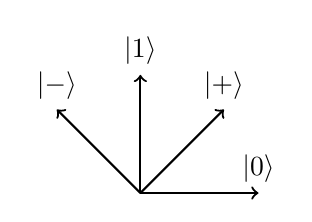
\begin{tikzpicture}[scale=1.5]
    \draw[->,thick] (0,0) -- (0,1) node [above] {$\ket{1}$};
    \draw[->,thick] (0,0) -- (1,0) node [above] {$\ket{0}$};
    \draw[->,thick] (0,0) -- (0.707,0.707) node [above] {$\ket{+}$};
    \draw[->,thick] (0,0) -- (-0.707,0.707) node [above] {$\ket{-}$};
\end{tikzpicture}
    \caption{Relative position of the basis in the quantum sharing case}
    \label{fig:shab}
\end{figure}
Assume that this is common knowledge, so initially the general state of the
system is $s = \alpha \ket{0} + \beta \ket{1}, |\alpha|^2 + |\beta|^2 = 0$.
Let us consider the initial announcement of the father. Note that as opposed to
the previous case, the two observations in this system \emph{cannot be measured
at the same time}. This is an instance of Heisenberg's uncertainty principle and
is due to the fact that the observations do not correspond to orthogonal
subspaces. So we cannot use the interpretation from the previous version here.
Suppose the father's announcement is: after observing Alice's face, it will
(possibly) become muddy, (classical) or, after observing Bob's face, it will
(possibly) become muddy. This corresponds to the condition $\beta \neq 0$ or 
$\alpha + \beta \neq 0$. But if $\beta = 0$, then necessarily $\alpha + \beta
\neq 0$ (since $s$ is a unit vector), thus this statement is true at every
state. So in this case, \emph{the father's initial announcement has no epistemic
(in terms of deletion of possible worlds) effect whatsoever}. Let us first
analyze the situation when this is the case.  After that we will argue that even
with a stronger initial announcement, the epistemic effect will essentially stay
the same.

First Alice observes Bob's face. That has the effect of collapsing the system
$s$ into the state $s' \in \{\ket{-}, \ket{+}\}$ (up to a unit complex
multiple). Any of these two states, if observed along the $\{\ket{0},\ket{1}\}$
basis, has an equal probability of $P = \frac{1}{2}$ to yield both answers.
Thus, Alice doesn't know (surely) if she would become muddy after observation or
not. But observe that she knows that \emph{she would become muddy after
observation with probability exactly $\frac{1}{2}$!} The situation for Bob is
symmetric: after observing Alice's face, he knows that he would become muddy
with probability exactly $\frac{1}{2}$. Observe that he knows that he had a
definite cleanness of himself right before he saw Alice's face, but the act of
observation of her face make his cleanness completely uncertain! Now that is a
truly quantum effect that we observe in this situation. After the first
observation, the system will always be in a state corresponding to some of the
four basis vectors and will always truly randomly transition to the next state.
So, even if the father announced for the initial system that either (surely)
Alice would become muddy or (surely) Bob would become muddy, this just amounts
to the condition $s \in \{\ket{1}, \ket{+}\}$, and will not change the epistemic
situation further. We saw that learning the probabilities of outcomes of
observations follows naturally from shared quantum behaviours.

\section*{Electron spin mud}

\begin{thebibliography}{9}
    \bibitem{corrkn}
    A. Baltag and S. Smets. “Correlated Knowledge, An Epistemic-Logic View on Quantum Entanglement", International Journal of Theoretical Physics
\end{thebibliography}

\end{document}
